\documentclass{article}
% arXiv preprint format, using the standard arxiv.sty. This is the extended
% version: no page limit, so it carries the explanatory figures and the longer
% derivations that the conference version (paper_iclr.tex) has to leave out.
\usepackage{arxiv}
\usepackage[utf8]{inputenc}
\usepackage[T1]{fontenc}
\usepackage{amsmath,amssymb}
\usepackage{graphicx}
\usepackage{booktabs}
\usepackage{caption}
\usepackage{url}
\usepackage[colorlinks=true,linkcolor=black,citecolor=black,urlcolor=blue]{hyperref}
\usepackage{xcolor}

\captionsetup{font=small,labelfont=bf,skip=6pt}

\newcommand{\keyfinding}[1]{\vspace{2pt}\noindent\fbox{\parbox{0.97\linewidth}{#1}}\vspace{2pt}}

\title{A Memory That Only Looks Like One:\\
A Hybrid Vision-Language Model Relays\\
the Picture Rather Than Storing It}

\author{Raj Dandekar \quad Rajat Dandekar \quad Sreedath Panat\\[3pt]
Vizuara AI Labs\\
\texttt{research@vizuara.com}}
\date{August 2026}

\renewcommand{\headeright}{Preprint}
\renewcommand{\undertitle}{Preprint, extended version}

\begin{document}
\maketitle

\begin{abstract}
\noindent
A hybrid vision-language model carries two kinds of memory. Its attention
layers keep a growing cache: every token the model reads, including every
patch of an image, is stored as a key-value entry that later tokens can look
up. Its recurrent layers keep a single state of fixed size, and every new
token overwrites part of that state. Prior work proved that a fixed-size state
must eventually lose information. But it does not tell us \emph{when} a given
model forgets, \emph{what} it keeps while forgetting, or \emph{what breaks}
downstream. We answer these three questions for Zamba2-VL-7B, a model in which
all 81 decoder layers carry a Mamba2 recurrent mixer and only 13 also carry
attention. Put simply: while the model talks about other things, where does
the picture live?

First, what does the recurrent state hold just after it reads an image? It
holds the gist, not the details. A linear probe reads \emph{which} object was
in the picture at $92.5\%$ accuracy from the best single layer, against a
$12.5\%$ chance rate. The same probe can barely read \emph{how many} objects
there were, or \emph{where} they sat.

Second, how fast should that memory fade? For this architecture the answer can
be computed from the weights alone, with nothing fitted. Mamba2 multiplies its
state by $\exp(\Delta_t A)$ at every token, so retention after $k$ tokens is
$\exp(A\sum\Delta_t)$, and each head has a half-life of
$\ln 2/(|A|\bar{\Delta})$ tokens. The median half-life is $6.6$ tokens in the
7B model, and $2.9$ and $2.6$ in its two smaller siblings. The weights say the
recurrent trace of the picture should be gone within a few tokens. (This
calculation predicts which heads depend on attention, but it does not predict
the measured decodability curve across scales; we report that failure.)

Third, and this is the central result: the memory a probe appears to find at
longer distances is mostly not memory. We split heads into fast-decaying and
slow-decaying groups while holding write strength fixed; the same gate
controls both, so a naive split confounds them. The ordering comes out exactly
as decay predicts, with slow heads reading better at every distance. But the
amounts are impossible. Heads with a $2.3$-token half-life still decode the
object at $26.6\%$ sixty-four tokens after the image, where their own
parameters retain $4\times10^{-9}$ of what was written. Something must be
re-supplying them. To find out what, we delete the image's key-value entries
from all 13 attention layers immediately after the image, without touching any
recurrent state. The apparent memory collapses: the fast third of heads falls
from $51.6\%$ to $7.8\%$ at thirty-two tokens, below chance. At matched write
strength the deletion costs fast heads $2.4$ times more than slow heads,
exactly the pattern a relay predicts. The recurrent channel is passing along
what attention still holds; it is not storing the picture.

A direct causal test agrees. We swapped the entire recurrent memory, all 81
states, between two runs that saw different images. Nothing changed: 100 of
100 answers still followed the run's own image, with every swap verified.
Swapping seven of the thirteen attention caches flipped 94 of 100 answers to
the other image. Finally, the practical consequence for cache pruning: on this
model, keeping a quarter of the visual key-value entries is safe at every
distance we tested, but below that the cost grows with distance. Removing every
visual entry costs $34$ accuracy points next to the image and $59$ points
thirty-two tokens later.
\end{abstract}

\begin{figure}[t]
\centering
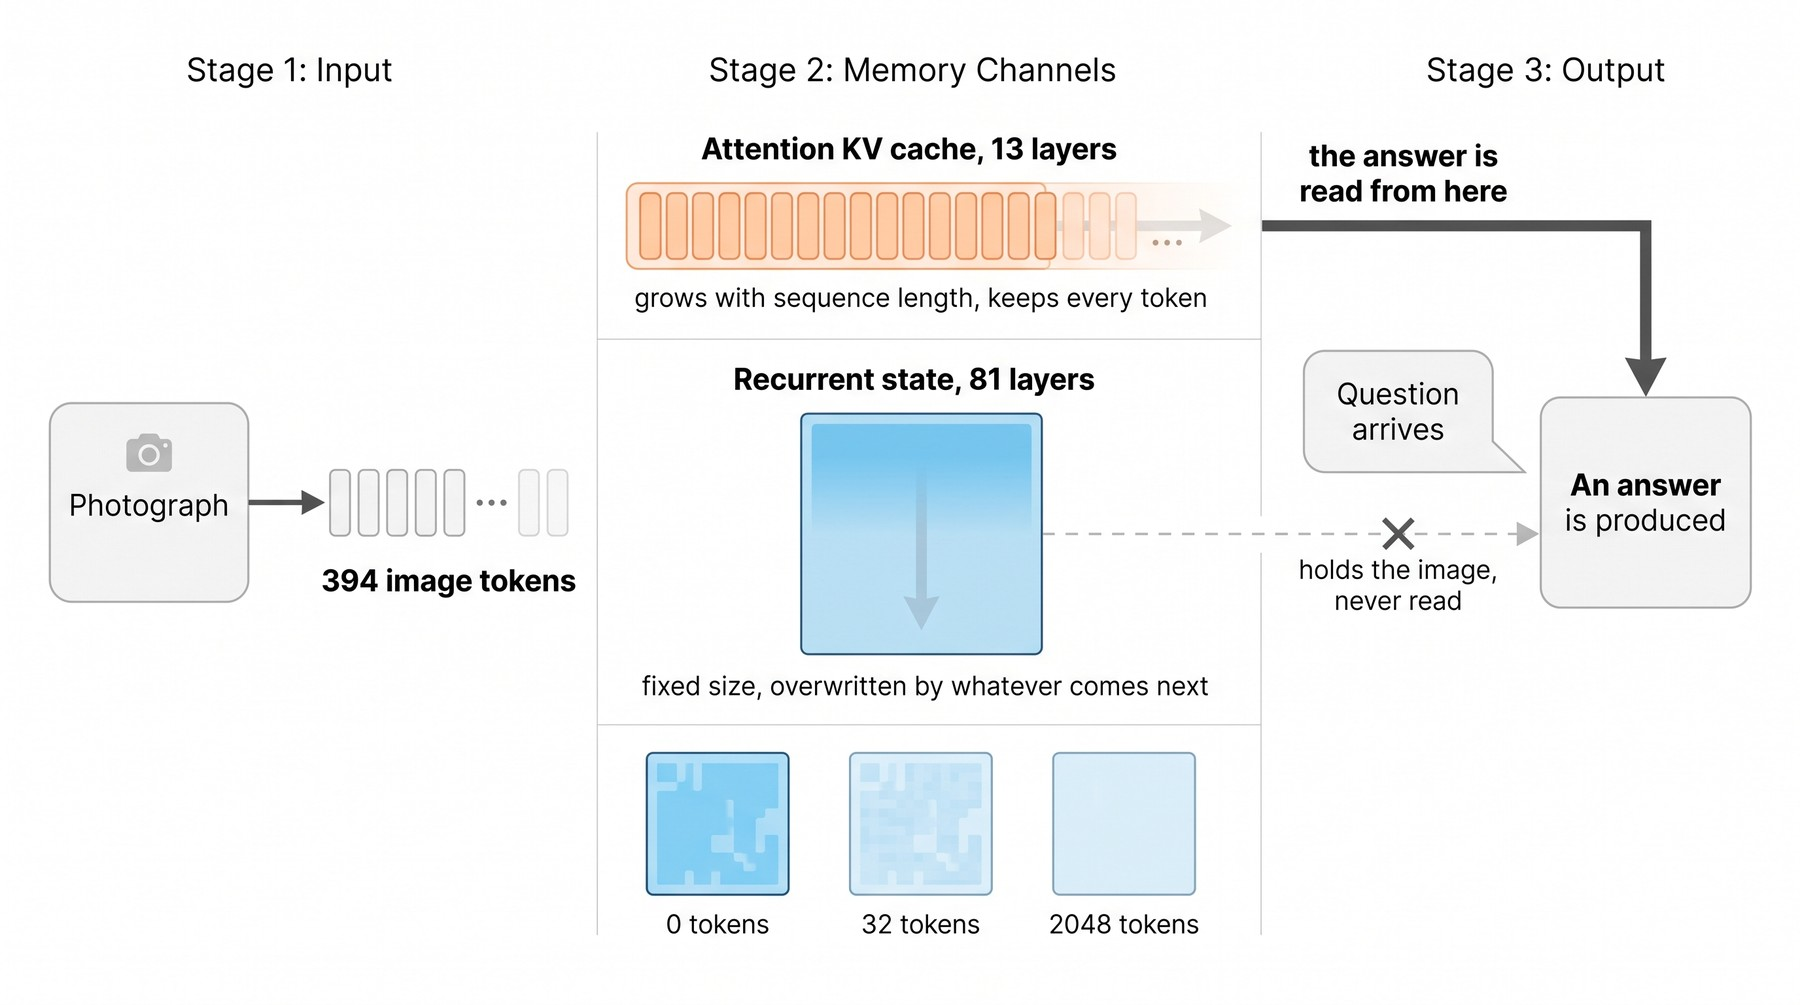
\includegraphics[width=0.94\linewidth]{assets/fig_idea.jpg}
\caption{The two memory channels of a hybrid vision-language model and the
question this paper asks of them.}
\end{figure}

\section{What Was Known Before, and What Is New Here}

Linear-attention and state-space models replace the growing key-value cache of
a transformer with a state of fixed size
\cite{katharopoulos2020linear,gu2022s4,peng2023rwkv,gu2023mamba,dao2024mamba2,beck2024xlstm}.
A fixed state cannot grow with the context. For this reason, most deployed
systems keep a few attention layers alongside the recurrent ones, and these
hybrid models are now common
\cite{lieber2024jamba,glorioso2024zamba,de2024griffin,ren2025samba,waleffe2024empirical}.
This paper asks a simple question about such a model: what is the recurrent
half actually holding?

We want to be clear about what is already known. Prior work established that a
fixed-size recurrent state must eventually lose information from context; that
premise is not ours. Jelassi et al.\ \cite{jelassi2024copying} prove that
transformers can copy exponentially long strings while state-space models are,
in their words, ``fundamentally limited by their fixed-size latent state''.
They also show empirically that pretrained transformers ``dramatically
outperform state space models at copying and retrieving information from
context''. Other results reach the same conclusion from other directions.
State-space models are limited to $\mathrm{TC}^0$ and cannot reliably track
state \cite{merrill2024illusion}. In-context retrieval is the specific skill
that separates recurrent models from transformers \cite{wen2024rnns}. Most of
the quality gap between efficient architectures and attention comes from
recall \cite{arora2023zoology,arora2024based}. Our work builds on these
results; it does not rediscover them.

Table~\ref{tab:novelty} states what that literature establishes and what this
paper adds.

\begin{table}[h]
\centering\small
\begin{tabular}{p{0.44\linewidth}p{0.48\linewidth}}
\toprule
\textbf{Established by prior work} & \textbf{New here} \\
\midrule
A fixed-size state must lose information from context, with a capacity proof
and behavioural evidence \cite{jelassi2024copying,merrill2024illusion,wen2024rnns}.
& \emph{When}. A retention horizon in tokens, computed from the model's own
$A$ and $\Delta$ with nothing fitted, at three scales. \\
\addlinespace
Recurrent models underperform at copying and retrieval as a class
\cite{arora2023zoology,arora2024based}.
& \emph{What survives}. The failure is content-selective: object identity is
highly decodable at the same instant that count and position are near chance. \\
\addlinespace
Architectures are compared to one another from the outside.
& \emph{Causal localisation inside one model}, and the finding that the
recurrent channel relays rather than stores, which makes probing it at distance
a measurement of the attention channel. \\
\addlinespace
Visual tokens and key-value entries carry substantial redundancy that can be
pruned \cite{chen2024fastv,yang2024visionzip,shang2025prumerge}.
& \emph{What underwrites that premise}, and that its safety margin shrinks
with distance from the image on a hybrid. \\
\bottomrule
\end{tabular}
\caption{Delineation of prior work and contribution.}
\label{tab:novelty}
\end{table}

\section{Significance}

Why does this matter? Hybrid models are being adopted because a fixed-size
state promises constant-memory inference. Anyone building or deploying one
must then decide how much to trust the recurrent channel: can it be relied on
to carry information across a long prompt? Today that is a judgement call.
This paper turns it into a calculation. Given a checkpoint's decay weight $A$
and its gate statistics, you can compute how many tokens the recurrent state
retains what it wrote, before running any experiment. For Zamba2-VL-7B the
answer is single digits. That is far shorter than one would guess from the
size of the state, which is $458{,}752$ numbers per layer.

There is also a concrete consequence for a popular optimization. A large body
of work speeds up vision-language models by discarding visual tokens or
evicting their key-value entries. The stated premise is that those entries are
largely redundant \cite{chen2024fastv,yang2024visionzip,shang2025prumerge}; a
parallel line evicts key-value entries in language models on similar grounds
\cite{zhang2023h2o,li2024snapkv,xiao2024streaming}. These methods were
developed and validated on dense transformers, where they work. We find that
they mostly survive the move to this hybrid: keeping a quarter of the visual
entries holds accuracy at every distance we tested. What does not survive is
the safety margin. The redundancy exists because the recurrent channel is
relaying the picture, and it only relays for a few tokens. As a result, the
cost of aggressive pruning roughly doubles between a prompt that asks about
the image immediately and one that asks thirty-two tokens later. A pruning
method tuned on short prompts will therefore look safer than it is. That is
the kind of failure a standard benchmark is least likely to catch.

\section{The Two Memories a Hybrid Carries}

A transformer remembers by accumulation. Every token it reads leaves a key and
a value in a cache, and every later token may attend to all of them. Nothing
is lost and nothing decays. The cost is that the cache grows with the context.
This growth is why serving long inputs is expensive.

A linear-attention or state-space layer remembers by summary. It keeps one
state of fixed size and updates it at every token, so its memory cost does not
grow at all. The cost appears somewhere else. The state is the same size after
ten tokens as after ten thousand, so everything it holds must share that
space. What a later token writes displaces what an earlier one wrote.

A hybrid model runs both at once. In Zamba2-VL-7B, all 81 decoder layers carry
a Mamba2 mixer with such a state, and 13 of them also carry an attention block
with an ordinary growing cache. Figure~\ref{fig:channels} draws the situation
at the moment the model is asked a question about an image it read $d$ tokens
earlier. The attention channel still holds the image exactly as it was read,
because nothing has removed those entries. The recurrent channel holds
whatever survives after $d$ rounds of overwriting.

Notice that the two channels give conflicting hints about where the picture
should be. The recurrent channel is much larger: 81 states of $458{,}752$
numbers each, $37{,}158{,}912$ numbers in total, against 13 caches holding a
few hundred entries apiece. If capacity decided the question, the picture
would be in the recurrent channel. But the recurrent channel is also the one
that overwrites itself. The architecture alone cannot tell us which channel
the model actually answers from. The rest of this paper settles the question
by experiment.

\begin{figure}[h]
\centering

\includegraphics[width=\linewidth]{assets/e4_two_channels.png}
\caption{The two memories at the moment the question arrives. \textbf{Top:}
the token stream, an image of 345 to 415 tokens followed by $d$ tokens of
filler and then the question. \textbf{Middle:} the attention channel appends
one key-value entry per token and keeps all of them, so the image is still
there when the question is asked. \textbf{Bottom:} the recurrent channel is
the same $458{,}752$ numbers per layer at every position, rewritten at every
token, so what the image wrote fades as the filler streams past. The question
this paper answers is whether it fades on the schedule the weights dictate.
Schematic; the quantities are those of Section~\ref{sec:model}.}
\label{fig:channels}
\end{figure}

\section{Model and Instruments}
\label{sec:model}

\subsection{The model}

Zamba2-VL-7B \cite{zamba2vl} is the vision-language member of the Zamba family
\cite{glorioso2024zamba}, which pairs a Mamba2 backbone \cite{dao2024mamba2}
with a shared attention module, and it takes its vision encoder from Qwen2.5-VL
\cite{bai2025qwen25vl}. It is Apache-2.0 licensed and has 81 decoder layers. Every one carries a Mamba2
mixer, and 13 of them additionally carry a shared attention block, at layer
indices 6, 11, 17, 23, 29, 35, 41, 47, 53, 59, 65, 71 and 77. The recurrent
channel therefore spans all 81 layers and the attention channel spans 13. Each
layer's recurrent state is a tensor of shape $[112, 64, 64]$, which is
$458{,}752$ numbers. One image occupies between 345 and 415 tokens depending on
its aspect ratio.

\subsection{Reading the state}

The Mamba2 recurrence is
\begin{equation}
S_t = S_{t-1}\exp(\Delta_t A) + \Delta_t\, x_t B_t^{\top},
\qquad y_t = S_t C_t ,
\end{equation}
so writing uses $(x, B)$, reading uses $C$, and retention of anything already
present is governed by $A$ and $\Delta$ alone.

Let us read that update in words, because everything in this paper follows
from it. At each token, two things happen to the state. First, it is
multiplied by $\exp(\Delta_t A)$, a number strictly between zero and one.
Second, the term $\Delta_t x_t B_t^{\top}$ is added to it. The multiplication
is the only operation that ever removes information: it shrinks everything the
state already held, uniformly, by a factor the model sets through the stored
weight $A$ and the input-dependent gate $\Delta_t$. The addition is the only
operation that ever writes. Reading the state, through $C_t$, changes nothing.

In other words, each head is a leaky accumulator, and its leak rate can be
computed in advance. Multiplying by $\exp(\Delta A)$ once per token for $k$
tokens leaves $\exp(A\sum_t\Delta_t)$ of whatever was there. Half of the
content is gone after $\ln 2/(|A|\bar{\Delta})$ tokens, so we call this
quantity the head's half-life. Notice what the expression does \emph{not}
contain: nothing about the image, the task, or the probe. It is one stored
weight and one gate statistic, and both can be read off a checkpoint before
any experiment is run. Section~\ref{sec:horizon} tests this prediction.

We verified each of these
against the installed model source rather than assuming the canonical form.
In particular $A = -\exp(A_{\log})$ is a per-head scalar, the gate is
$\Delta = \mathrm{softplus}(\Delta_{\text{raw}} + b)$ clamped below at
$0.001$ with no upper clamp, and the decay factor is
$\exp(\Delta_t A)$ elementwise.

To measure what the state holds, we use a linear probe. A linear probe is the
simplest possible reader: a classifier that computes a weighted sum of the
state's numbers and predicts the trial's answer from that sum alone, with no
other computation. We train it on some trials and test it on held-out ones.
If even this simple reader recovers the answer, the answer is present in the
state in an easily readable form. Probing a representation this way is
standard \cite{alain2016probes}, and its hazards are well known. A probe can
succeed because the classifier is powerful, not because the model uses the
information. This is why probing papers check selectivity against control
tasks \cite{hewitt2019control} and read their results with care
\cite{belinkov2022probing}. We therefore never rely on a probe alone. Every
probe result in this paper is paired with an intervention on the model, in the
tradition of causal mediation analysis \cite{vig2020causal} and activation
patching \cite{meng2022rome,wang2022ioi,zhang2024patching}, and we follow that
literature's recommendation to report what each intervention does to the
model's own behaviour, not only to the probe's readout \cite{zhang2024patching}.

One practical detail: $458{,}752$ numbers per layer is too wide to probe
directly, so each layer's state is first passed through a fixed Gaussian random
projection down to 512 features. By the Johnson-Lindenstrauss property, such a
projection preserves linear separability up to a controlled distortion. A
linear probe on the projected features is therefore, to that tolerance, a
linear probe on the state itself. The projection columns are drawn
independently, so the first $k$ columns form a valid $k$-feature projection on
their own.

Probes are ridge classifiers evaluated by block-grouped $k$-fold
cross-validation, with the ridge penalty chosen on inner training folds only.
One rule matters enough to state on its own: every probe is fitted and
evaluated \emph{within a single condition}. A probe reported for the evicted
condition is trained only on evicted trials and tested on held-out evicted
trials. It is never trained on intact trials and applied to evicted ones. Why
does this matter? If we had transferred a probe across conditions, a
below-chance readout would be the expected signature of a distribution shift
between conditions, and it would tell us nothing about what information is
present. Because each condition supplies its own training and test folds, a
drop under eviction means one thing: less linearly decodable information in
that condition. The below-chance cells reported later are within sampling
noise at these sample sizes. A reading of $7.8\%$ is 5 correct out of 64
($P(X \le 5) = 0.17$ under the null), and $4.7\%$ is 3 of 64 ($P = 0.034$), so
across twenty cells roughly three readings below chance are expected by
chance alone.

\subsection{Splicing the channels}

The splice experiment runs the model twice, on two different images, and then
physically exchanges one memory channel between the two runs while leaving the
other channel untouched. The run that keeps its own question is called the
host; the run that donates its memory is called the donor. After the exchange,
the host answers its question, and we record whose image the answer describes.
Swapping the recurrent channel replaces all 81 states and convolution buffers.
Swapping the attention channel replaces the 13 key and value caches. The
host's cache is restored exactly afterwards, so one prefill supports many
conditions.

\subsection{The three experiments in one picture}

Three protocols recur throughout the paper, and Figure~\ref{fig:protocols}
shows what each one does to a run. The first is the probe: read the recurrent
state just before the question, and measure what is linearly present at a
chosen distance. The second is the eviction: delete the image's key-value
entries from all 13 attention layers at the moment the image finishes, before
a single filler token is processed, and then probe the state exactly as
before. At the instant of the deletion, the recurrent state is identical in
both runs. Any difference that appears later must therefore come from the
attention channel. The third is the splice described above, which measures
which channel the model's own answer follows.

\begin{figure}[h]
\centering

\includegraphics[width=\linewidth]{assets/e5_protocols.png}
\caption{The three protocols. \textbf{1:} a linear probe reads the recurrent
state at the position just before the question; the task is eight-way forced
choice, so chance is exactly $12.5\%$. \textbf{2:} the image's attention entries
are deleted at the moment the image ends, before any filler token is processed,
leaving the recurrent state untouched and identical to the intact run at that
instant. \textbf{3:} one channel is exchanged between two runs that saw
different images, and the host run's question is then asked. Schematic.}
\label{fig:protocols}
\end{figure}

\section{Materials}

Trials are built from COCO val2017 instance annotations \cite{lin2014coco},
the corpus underlying most visual instruction tuning \cite{liu2023llava}.
There are three question families: which object is present, how many of a
named object are present, and where in the picture a named object is. Every
question is eight-way forced choice, so the chance rate is exactly $12.5\%$.
Trials are constructed in blocks of eight. All eight trials in a block share
one identical candidate list, and each candidate is the correct answer exactly
once within the block. This construction is what makes the pre-image control
meaningful. Because the candidate set is fixed and each answer appears
equally often, a classifier that has not seen the image has nothing to
exploit: no candidate is more likely than any other, so it cannot beat
chance.

Images are fetched at native geometry for the decay experiments. For the splice
they are letterboxed onto a common square canvas, because two runs on images of
different shape emit different numbers of vision tokens and therefore
different-length attention caches, which cannot be exchanged. Letterboxing
rather than square resizing matters: in a pilot, a plain square resize deformed
the content enough to halve identity accuracy, so every splice image is
letterboxed.

\section{Result 1: The State Records Gist, Not Particulars}

We first probe the state at distance zero, the instant the image has just
been read. The state is highly informative about which object is present, and
close to uninformative about how many objects or where they are. The best
single layer reads identity at $92.5\%$ against the $12.5\%$ chance rate. A
probe given all 81 layers at once reads identity at $83.1\%$
($p = 6 \times 10^{-92}$, $n = 160$), count at only $19.4\%$ ($p = 0.009$),
and position at only $17.5\%$ ($p = 0.041$). Note that the all-layer figure is
pulled down by overfitting, because it fits $41{,}472$ features to 120 trials.
We therefore use it only to compare the three properties against each other,
never as a measure of how much the state holds.

In fact these figures understate what the state carries. The full-state
feature vector has $81 \times 512 = 41{,}472$ dimensions, far more than the
number of trials, and a probe on a single layer does substantially better.
Layer 64 alone reads identity at $92.5\%$. The last 21 layers (60 to 80)
average $85.2\%$, against $59.0\%$ for the middle third of the stack (layers
27 to 53). On the identical trials, the full-state probe reads $71.7\%$. Two
conclusions follow. The gist is stronger than the aggregate number suggests,
and it is concentrated in the late layers, as the right panel of
Figure~\ref{fig:horizon} shows.

\begin{figure}[h]
\centering

\includegraphics[width=\linewidth]{assets/f1_horizon_depth.png}
\caption{\textbf{Left:} identity decoded from the recurrent state against
distance from the image, at three model scales, 120 trials per point. The
pre-image control reads exactly $12.5\%$ at every scale. \textbf{Right:}
identity decoded from each layer's state alone at the instant of writing, with
red marking the 13 layers that also carry attention. A probe given all 81 layers
at once does worse than the best single layer, because $41{,}472$ features on
120 trials is heavily overparameterised.}
\label{fig:horizon}
\end{figure}

\keyfinding{The recurrent state is not a compressed copy of the image. It is a
selective summary that keeps object identity and discards count and position, and
that selection is visible at the instant of writing rather than emerging over
distance.}

\section{Result 2: The Forgetting Horizon, Predicted From the Weights}
\label{sec:horizon}

\subsection{The prediction}

Retention of whatever the state held, after $k$ further tokens, is
\begin{equation}
R(k) = \exp\!\Big(A \sum_{t=1}^{k}\Delta_t\Big),
\qquad
\text{half-life} = \frac{\ln 2}{|A|\,\bar{\Delta}} .
\end{equation}
$A$ is a stored weight. $\bar{\Delta}$ is measured from the gate channels of
the input projection, over the tokens that follow the image, on the same
prompts the decay experiment uses. Nothing here is fitted to a decay curve.

Across all $81 \times 112 = 9{,}072$ heads, the predicted median half-life is
$6.6$ tokens, with an interquartile range of $2.8$ to $17.8$. $85.0\%$ of
heads fall below 32 tokens, and only $0.08\%$ exceed 512.
Figure~\ref{fig:halflife} draws the full distribution: a dense cluster of
heads in the single digits, plus a thin tail of slow heads reaching past a
hundred tokens. Keep that tail in mind. When a probe still reads something at
long distance, the most natural explanation is that this slow minority
carries it. Section~\ref{sec:relay} tests that explanation directly and finds
it insufficient: the slow heads do keep more, but nowhere near enough to
explain the readings.

\begin{figure}[h]
\centering

\includegraphics[width=\linewidth]{assets/e1_halflife_distribution.png}
\caption{\textbf{Left:} predicted half-life for each of the $9{,}072$ heads of
Zamba2-VL-7B, from that head's own $A$ and its mean gate over the filler.
The median is $6.6$ tokens and $85\%$ of heads fall below 32.
\textbf{Right:} the same quantity at three model scales, as the share of heads
whose half-life falls below a given value. The distributions differ in detail
but not in kind; at every scale the bulk of the model forgets within tens of
tokens.}
\label{fig:halflife}
\end{figure} Measured over eight different
photographs the median moves only between $6.44$ and $6.86$ tokens, so the
horizon is a property of the model rather than of the stimulus.

\subsection{The measurement}

Does the measured decay match this prediction? Our original collection
measured only distances $0$ and $32$, and $32$ tokens is already far past the
region where the prediction changes quickly. Table~\ref{tab:fine} therefore
shows a finer sweep, on 120 identity trials at each of eleven distances.

\begin{table}[h]
\centering\small
\begin{tabular}{rrrrr}
\toprule
tokens & probe accuracy & $p$ & behaviour & predicted retention (median) \\
\midrule
0  & $71.7\%$ & $2\times10^{-50}$ & $94.2\%$ & $1.000$ \\
1  & $60.0\%$ & $2\times10^{-34}$ & $96.7\%$ & $0.901$ \\
2  & $59.2\%$ & $2\times10^{-33}$ & $97.5\%$ & $0.812$ \\
4  & $41.7\%$ & $1\times10^{-15}$ & $96.7\%$ & $0.659$ \\
8  & $35.0\%$ & $2\times10^{-10}$ & $97.5\%$ & $0.434$ \\
12 & $30.0\%$ & $3\times10^{-7}$  & $96.7\%$ & $0.286$ \\
16 & $24.2\%$ & $3\times10^{-4}$  & $97.5\%$ & $0.188$ \\
24 & $29.2\%$ & $1\times10^{-6}$  & $95.8\%$ & $0.082$ \\
32 & $20.8\%$ & $7\times10^{-3}$  & $95.0\%$ & $0.036$ \\
48 & $25.8\%$ & $6\times10^{-5}$  & $97.5\%$ & $0.007$ \\
64 & $21.7\%$ & $3\times10^{-3}$  & $98.3\%$ & $0.001$ \\
\bottomrule
\end{tabular}
\caption{Decodability of object identity against distance from the image, on
120 trials at every distance, with the retention predicted from the weights
alongside. Chance is $12.5\%$, and the pre-image control reads exactly
$12.5\%$. Notice the shape: the reading falls fast, as the weights predict,
and then stops well short of chance. At 64 tokens the predicted retention is
$0.001$ of the trace, yet the probe still reads $21.7\%$. That tension is
resolved in Section~\ref{sec:relay}. Notice also the behaviour column: the
model itself answers correctly at every distance throughout.}
\label{tab:fine}
\end{table}

The measured signal halves at $4.0$ tokens, which falls inside the predicted
interquartile range of $2.8$ to $17.8$. Normalised to its value at distance
zero, measured decodability correlates with predicted mean retention at
$r = 0.973$ across the eleven distances, with no free parameters.
Figure~\ref{fig:retention} shows both halves of this comparison. The left
panel is the prediction on its own: three retention curves, one per stratum,
each produced by multiplying by $\exp(-|A|\bar{\Delta})$ once per token and
doing nothing else. The right panel compares that prediction with what the
probe actually read, distance by distance.

\begin{figure}[h]
\centering
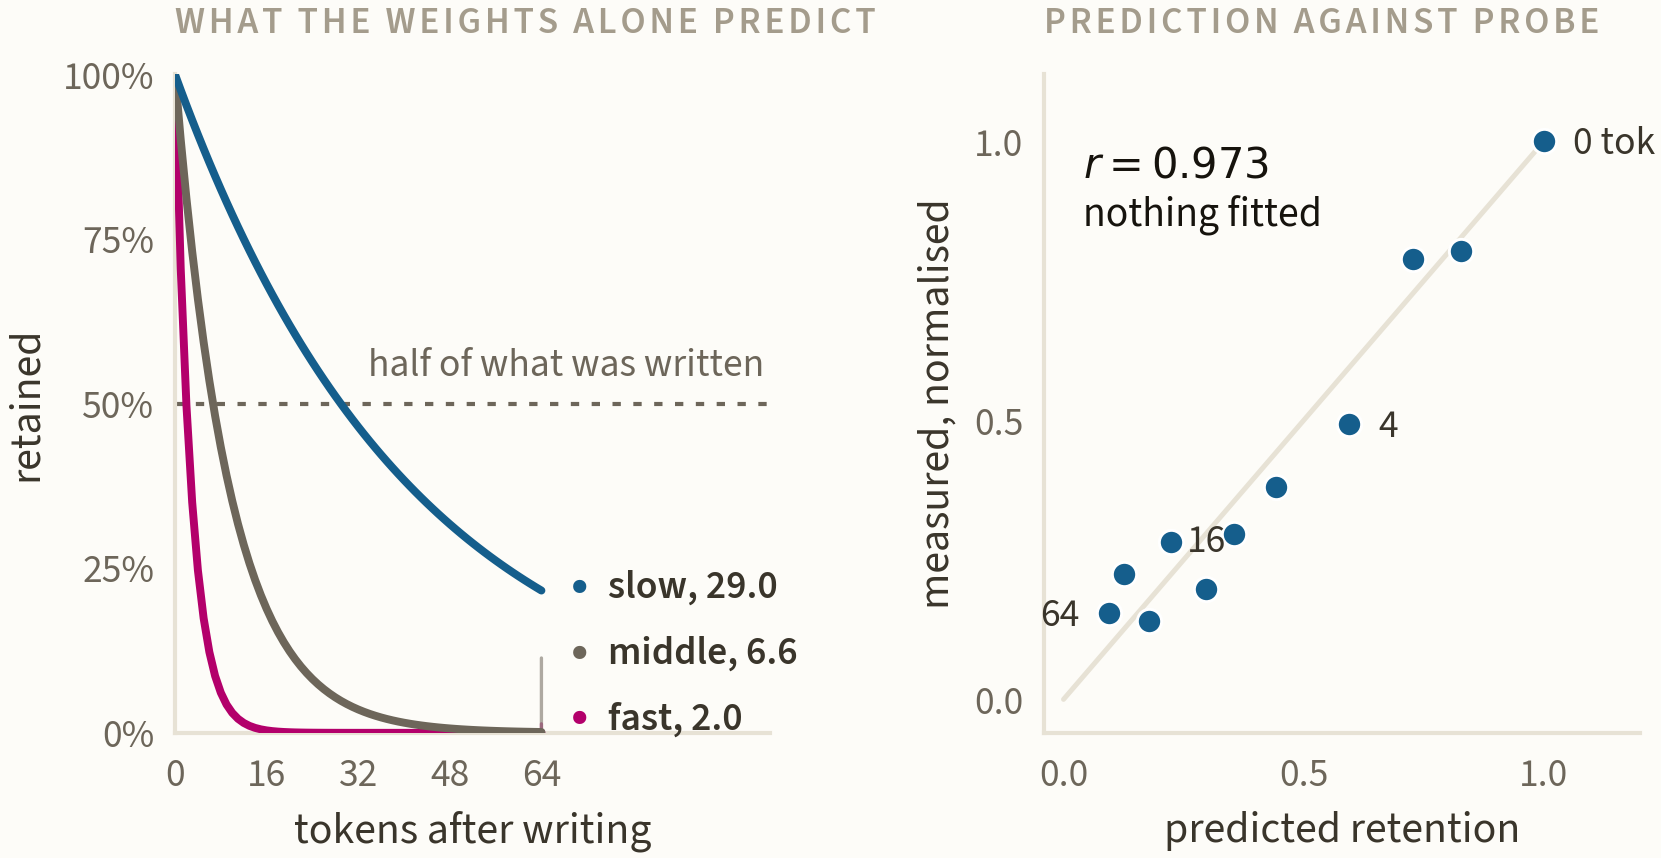
\includegraphics[width=\linewidth]{assets/e3_retention_curves.png}
\caption{\textbf{Left:} what the weights alone predict. Each curve is
$\exp(-|A|\bar{\Delta}k)$ at the median rate of one third of the heads, labelled
with that third's median half-life. Nothing is fitted. \textbf{Right:} predicted
retention against measured decodability, normalised to distance zero and
labelled by distance in tokens. The agreement on this model is $r = 0.973$.
Section~\ref{sec:scale} reports that it does not replicate across scales, and
Section~\ref{sec:relay} explains why it cannot.}
\label{fig:retention}
\end{figure} Beyond 16
tokens the measured curve sits above the predicted median and between the median
and the mean, which is what the heavy tail of slow heads predicts: the residual
signal at long distance is carried by the minority of heads with long
half-lives.



Throughout this collapse the model's own accuracy never moves. It answers
correctly on $94$ to $98\%$ of trials at every distance, including those where
the state has been emptied.

\subsection{The within-model test, with write amplitude held fixed}
\label{sec:strata}

A curve comparison alone cannot rule out coincidence. So we ran a sharper
test. Every head has its own predicted half-life, so we can sort them. We
call a head \emph{fast} if its half-life is short, around two tokens, meaning
its state should empty almost immediately, and \emph{slow} if its half-life
is long, meaning it should hold information longest. We then probe the fast
group and the slow group separately, using the same projection basis so the
groups are comparable to each other and to the unstratified probe. If the
state is genuinely retaining, decay makes a clear prediction: the fast heads
should lose the image first, and whatever signal survives at long distance
should be carried by the slow heads.

Before giving the result, we must explain a confound, because it changed our
own conclusions. The half-life is $\ln 2/(|A|\bar{\Delta})$, and the gate
$\bar{\Delta}$ appears in the write term as well. The gate therefore does
double duty: it sets how fast a head forgets, and it also sets how strongly
the head writes, by about a factor of seven between the fastest and slowest
thirds. Why does writing harder matter? Because a head that writes with
larger numbers leaves a stronger signal in its state, and a stronger signal
is easier for a linear probe to read, regardless of where the information
came from or how old it is. Sorting heads by half-life therefore also,
accidentally, sorts them by signal strength. The naive split indeed produces
a striking reversal, with the fast third decoding identity at $61.7\%$ after
sixty-four tokens while the slow third falls to $16.7\%$, the opposite of the
decay ordering. That reversal has nothing to do with memory. It is the write
strength.

The fix is to compare only heads that write equally hard. We keep the
$3{,}628$ heads whose mean gate falls in the middle forty percent of its
distribution, so write strengths are nearly matched, and split those by the
decay weight $|A|$ alone. This gives two strata of $907$ heads each. Their
predicted median half-lives still differ sevenfold, $2.3$ against $16.4$
tokens, but their write gains are now nearly equal (median $\bar{\Delta}$ of
$0.074$ against $0.066$). The only meaningful difference between the two
groups is how fast they forget.

With the gate controlled, the reversal disappears (Table~\ref{tab:strata},
left panel of Figure~\ref{fig:relay}). The slow stratum decodes better at all
seven distances measured, and it keeps a larger fraction of its distance-zero
signal at sixty-four tokens, $0.28$ against $0.20$. The ordering that the
decay parameters predict is real; amplitude had been masking it.

\begin{table}[h]
\centering\small
\begin{tabular}{lrrrrrr}
\toprule
stratum & predicted $t_{1/2}$ & $d{=}0$ & $d{=}16$ & $d{=}32$ & $d{=}64$ & signal kept at $d{=}64$ \\
\midrule
fast & $2.3$  & $81.8\%$ & $50.0\%$ & $35.9\%$ & $26.6\%$ & $0.20$ \\
slow & $16.4$ & $91.7\%$ & $61.5\%$ & $46.9\%$ & $34.4\%$ & $0.28$ \\
\bottomrule
\end{tabular}
\caption{Identity decodability by gain-matched stratum, $n = 192$ per cell,
chance $12.5\%$. ``Signal kept'' is the above-chance excess at $d{=}64$ as a
fraction of the excess at $d{=}0$. The slow stratum keeps more at every
distance, which is the decay ordering; both strata keep far more than their
own decay parameters permit.}
\label{tab:strata}
\end{table}

\begin{figure}[h]
\centering
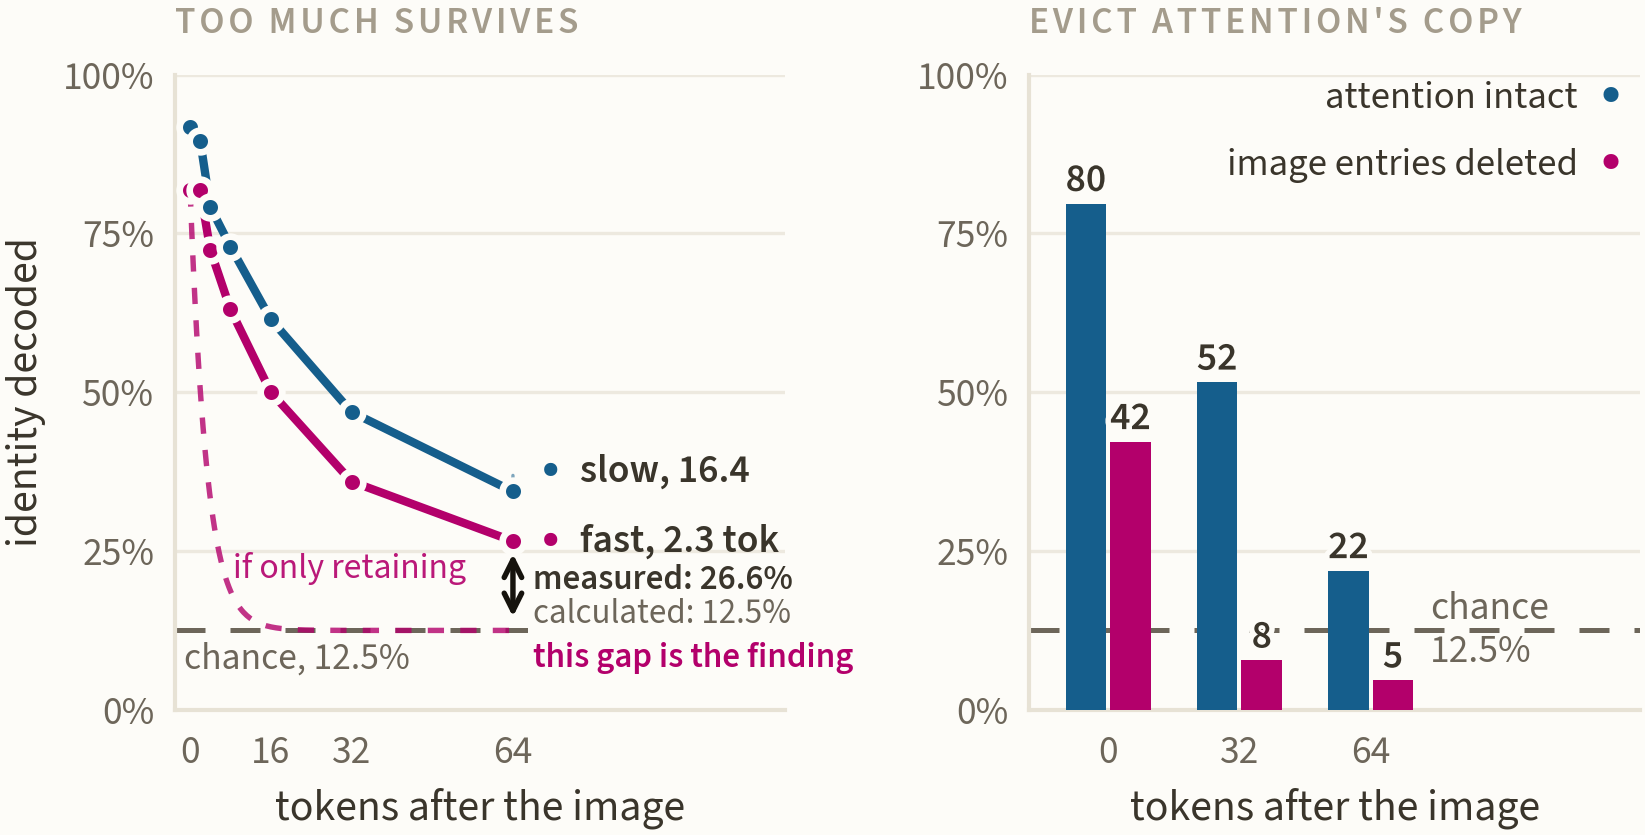
\includegraphics[width=\linewidth]{assets/f2_relay.png}
\caption{\textbf{Left: how to read this panel.} The two solid curves are
measurements: identity decoded from the slow stratum and from the fast
stratum at each distance, with write gain matched and $n = 192$ per point.
The dashed curve is not a measurement. It is a calculation: where the fast
stratum's reading would fall if it came only from what its own $2.3$-token
half-life retains. That calculated curve reaches chance within ten tokens;
the measured one ends at $26.6\%$ at $d{=}64$. The solid curves being
ordered slow-above-fast is what decay predicts; the gap between the two fast
curves is what decay cannot explain. \textbf{Right:} the same recurrent state
probed with and without the attention channel's copy of the image, fast
tercile, $n = 64$ per bar. The eviction happens immediately after the image
is read and never touches the recurrent state, which is identical in both
runs at that instant.}
\label{fig:relay}
\end{figure}

But now look at the amounts, because they are the finding. A stratum with a
predicted half-life of $2.3$ tokens retains
$2^{-64/2.3} \approx 4\times10^{-9}$ of anything it wrote sixty-four tokens
ago. Yet it reads $26.6\%$ there, twice the chance rate
($p = 1\times10^{-7}$, $n = 192$), and the measured half-life of its readout
is $19.3$ tokens, eight times its prediction. The slow stratum overshoots in
the same direction: predicted $16.4$ tokens, measured $26.3$, with four times
more signal surviving at $d{=}64$ than its parameters allow. In short, the
strata are ordered exactly as decay predicts, and both hold far more signal
than decay permits.

One caveat applies to any global split of this kind. Half-life varies across
the stack by almost two orders of magnitude (Figure~\ref{fig:bydepth}), from
a median of $1.7$ tokens at the fastest layer to $84.7$ at the slowest. A
global split by a decay quantity is therefore also a partial split by depth,
and depth matters for decoding. This affects the comparison \emph{between}
strata. It does not affect the comparison of each stratum with its own
prediction: whatever layers the fast stratum draws from, its own decay
parameters bound what it can retain, and it reads far above that bound.

\begin{figure}[h]
\centering
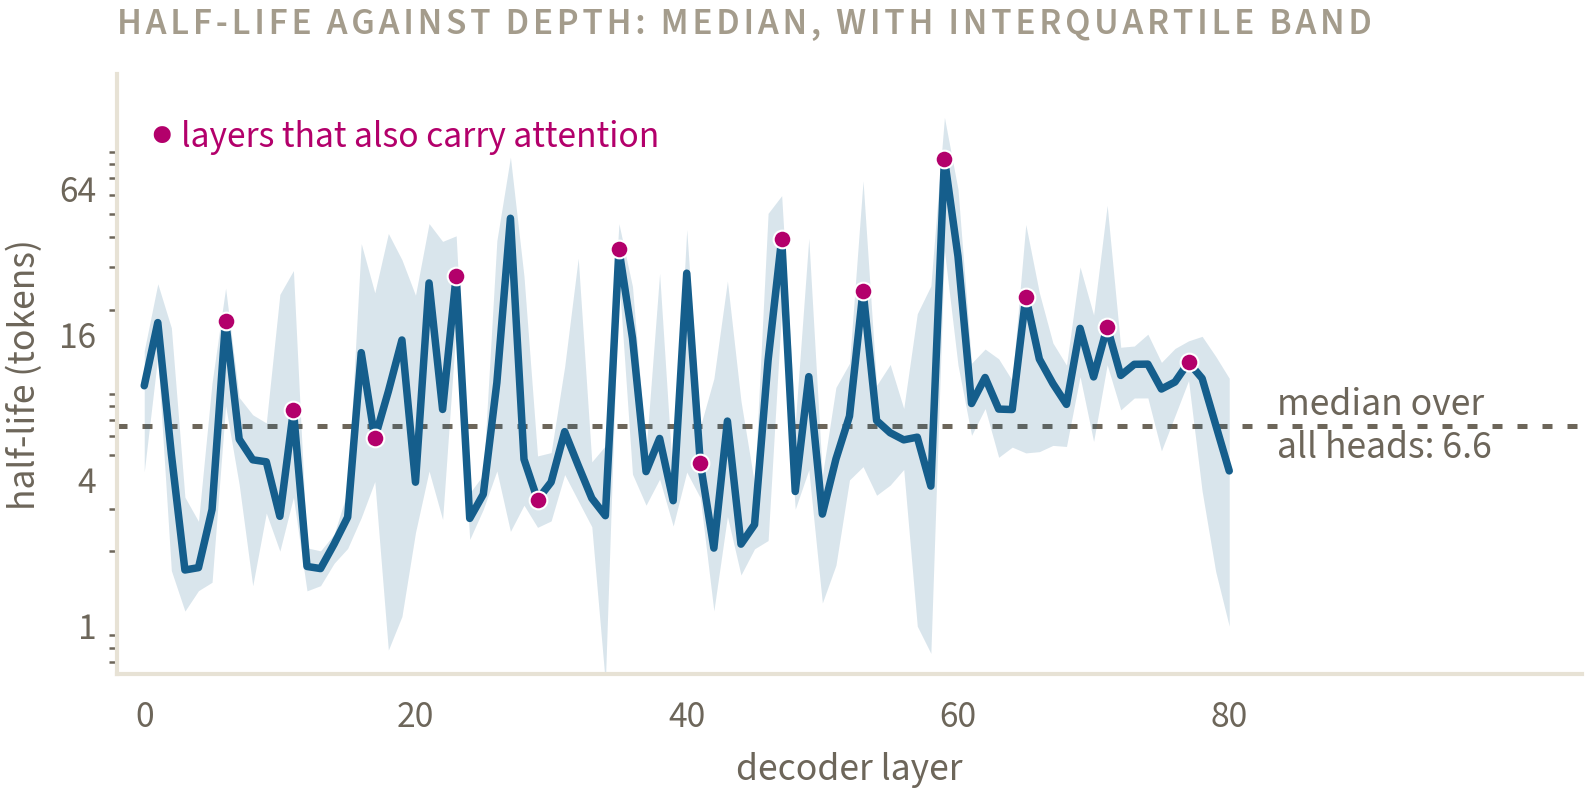
\includegraphics[width=\linewidth]{assets/e2_halflife_by_layer.png}
\caption{Predicted half-life against depth for Zamba2-VL-7B: the median over the
112 heads of each layer, with the interquartile band. The spread within a single
layer is often wider than the difference between layers, which is what makes a
global split by half-life only a partial split by depth. Red marks the 13 layers
that also carry attention.}
\label{fig:bydepth}
\end{figure}

\keyfinding{With write amplitude held fixed, the strata are ordered exactly as
decay predicts, and both hold far more signal than decay permits. A head with
a two-token half-life cannot be holding something written sixty-four tokens
earlier: by then its state consists almost entirely of recent writes. If such
heads still decode object identity at twice chance, the identity information
in their state arrived recently. Something else in the model must be supplying
it.}

\section{Result 3: The Recurrent Channel Is a Relay, Not a Store}
\label{sec:relay}

What could be supplying it? Only one component of the model still holds the
image at distance: the attention channel, whose key-value entries do not decay.
We tested this directly. Each trial was run twice, identically, except that in
one run we deleted the image's key-value entries from all 13 attention layers
immediately after the image was read, \emph{before a single filler token was
processed}. The deletion does not touch the recurrent state. At that instant,
the recurrent state is identical in both runs.

The two hypotheses now make opposite predictions. If the recurrent state is
remembering the image on its own, deleting attention's copy should not change
what a probe reads from the state. If the state is being refreshed from
attention, the deletion should collapse decodability at distance, and it
should hurt the fast heads most, because they depend most on being refreshed.

\begin{table}[h]
\centering\small
\begin{tabular}{lrrrr}
\toprule
stratum & distance & visual KV intact & visual KV evicted & change \\
\midrule
fast   & 0  & $79.7\%$ & $42.2\%$ & $-37.5$ \\
fast   & 32 & $51.6\%$ & $\mathbf{7.8\%}$  & $-43.7$ \\
fast   & 64 & $21.9\%$ & $4.7\%$  & $-17.2$ \\
\addlinespace
middle & 0  & $62.5\%$ & $43.8\%$ & $-18.8$ \\
slow   & 0  & $62.5\%$ & $54.7\%$ & $-7.8$  \\
\addlinespace
all    & 0  & $59.4\%$ & $59.4\%$ & $0.0$   \\
all    & 32 & $6.2\%$  & $6.2\%$  & $0.0$   \\
\bottomrule
\end{tabular}
\caption{Identity decodability from the recurrent state with and without the
attention channel's copy of the image, $n = 64$ per cell. Chance is $12.5\%$.
The fast heads' apparent memory at 32 tokens is entirely dependent on the
attention channel: removing it drops them from $51.6\%$ to below chance.}
\label{tab:relay}
\end{table}

\begin{figure}[h]
\centering

\includegraphics[width=\linewidth]{assets/f3_controls.png}
\caption{\textbf{Left: read this panel vertically.} At every position on the
x-axis, compare each curve with the no-eviction baseline. The text-eviction
curve sits above the baseline everywhere: deleting text raises the reading.
The image-eviction curve sits below it: deleting the image lowers the
reading. Both deletions remove the same number of positions from the same 13
caches, so damage alone cannot explain opposite signs. (All curves also slope
downward to the right; that is only because slower heads read less at this
distance in every condition.) \textbf{Right:} accuracy lost when the visual
entries are zeroed at all 13 attention layers, at only the earliest three,
and at only the latest three. The earliest three reproduce most of the full
effect; the latest three do nothing, so visual information enters early.}
\label{fig:controls}
\end{figure}

\subsection{Controls: the eviction removes the image, not merely positions}
\label{sec:controls}

There is a fair objection to the eviction experiment: the deletion changes
more than the image's presence. Removing the visual entries shortens every
attention cache by roughly 400 positions, and it changes the softmax
normalisation for every token that follows. Perhaps the readout collapsed
because we damaged the machinery, not because we removed a memory. Here is
the experiment that settles it. Run the deletion twice, on the same trials.
In one version, delete the image's entries, exactly as before. In the other,
delete the same \emph{number} of positions from the same caches, but delete
text instead of the image. Both versions do identical mechanical damage: the
same number of entries gone, the same shorter caches, the same disturbance to
attention. So if damage were the explanation, both versions should push the
reading down. We ran this control on ten strata formed by deciles of
predicted half-life, with 64 trials per cell (Table~\ref{tab:controls}).

That is not what happens. The two deletions move the readout in opposite
directions, shown in the left panel of Figure~\ref{fig:controls}. At 32
tokens, deleting the image costs the fastest decile $18.8$ points, while
deleting an equal number of the most recent pre-image text positions
\emph{raises} it by $29.7$ points. Averaged over the ten strata, the two
effects are $-6.4$ and $+12.5$ points. Deleting text plausibly helps because
the text was competing with the image for the residual stream, and removing
it leaves the image easier to relay. The key point is the signs. Identical
mechanical damage moves the reading in opposite directions, and damage cannot
push a reading up.
The same dissociation holds on the gain-matched strata at three times the
trial count ($n = 192$ per cell): deleting the image beside it costs the fast
stratum $22.4$ points while deleting matched text \emph{raises} it $13.5$,
and at thirty-two tokens text deletion raises the two strata by $31$ and $32$
points while image deletion moves them by $+1$ and $-7$.

\begin{table}[h]
\centering\small
\begin{tabular}{rrrrrrr}
\toprule
& & \multicolumn{3}{c}{$d = 0$} & \multicolumn{2}{c}{$d = 32$} \\
\cmidrule(lr){3-5}\cmidrule(lr){6-7}
decile & pred.\ $t_{1/2}$ & intact & evict image & evict text & intact & evict image \\
\midrule
1  & $0.70$ & $56.2\%$ & $18.8\%$ & $78.1\%$ & $31.2\%$ & $12.5\%$ \\
2  & $1.84$ & $56.2\%$ & $17.2\%$ & $79.7\%$ & $29.7\%$ & $12.5\%$ \\
3  & $2.75$ & $53.1\%$ & $18.8\%$ & $73.4\%$ & $20.3\%$ & $4.7\%$  \\
4  & $3.79$ & $46.9\%$ & $21.9\%$ & $71.9\%$ & $23.4\%$ & $15.6\%$ \\
5  & $5.38$ & $31.2\%$ & $26.6\%$ & $42.2\%$ & $12.5\%$ & $9.4\%$  \\
6  & $8.15$ & $35.9\%$ & $40.6\%$ & $51.6\%$ & $17.2\%$ & $20.3\%$ \\
7  & $11.8$ & $37.5\%$ & $25.0\%$ & $54.7\%$ & $10.9\%$ & $9.4\%$  \\
8  & $17.8$ & $45.3\%$ & $29.7\%$ & $57.8\%$ & $20.3\%$ & $18.8\%$ \\
9  & $32.0$ & $28.1\%$ & $26.6\%$ & $32.8\%$ & $15.6\%$ & $15.6\%$ \\
10 & $73.3$ & $51.6\%$ & $29.7\%$ & $46.9\%$ & $23.4\%$ & $21.9\%$ \\
\bottomrule
\end{tabular}
\caption{The matched-eviction control by decile of predicted half-life, $n = 64$
per cell, chance $12.5\%$. ``Evict image'' and ``evict text'' delete the same
number of positions from the same 13 attention caches. Single cells carry about
$6$ points of binomial noise at $n = 64$, and two of the twenty image-eviction
cells fall slightly the wrong way; the trend rather than any one cell is the
result. The drop under image eviction correlates with the decay rate
$1/t_{1/2}$ at $r = 0.647$ ($95\%$ CI $[0.03, 0.91]$) at $d{=}0$ and $r = 0.800$ ($[0.34, 0.95]$) at $d{=}32$. With ten strata these intervals are wide, and the lower bound at $d{=}0$ is close to zero.}
\label{tab:controls}
\end{table}

The same collection also tells us where the relayed information enters the
model, in the right panel of Figure~\ref{fig:controls}. Zeroing the visual
entries at only the three earliest attention layers reproduces $15.8$ of the
$17.2$ points lost when all thirteen are zeroed. Zeroing the three latest
layers costs only $0.5$ points. So visual information enters through the early
attention layers and is consumed downstream. (For these per-layer conditions
we zero entries rather than delete them, because Zamba2's attention blocks are
shared and accept a single mask length. Where both operations are available,
at $d{=}32$, they agree to within $2.34$ points, which validates the
substitution.)

Finally, the contrast is stable across the choice of projection basis. Repeating
it with three independent Gaussian projections gives, for the fast tercile at
$32$ tokens, intact $31.2 \pm 1.6\%$ against evicted $9.9 \pm 1.8\%$ (mean and
standard deviation over seeds), while the slow tercile shows no eviction effect
at any seed.

\subsection{The decay parameters predict how much is relayed}

Result 2 found that the parameter-derived horizon does not predict the
measured decodability curve. It does predict something else, and that
something is exactly what the relay account says it should predict. Reason it
through: a head that forgets quickly must depend more heavily on being
refreshed, so deleting the source of the refresh should hurt its readout
more. Ordering the strata by decay rate shows exactly this pattern. The size
of the effect depends on how the strata are formed:

\begin{table}[h]
\centering\small
\begin{tabular}{llrrr}
\toprule
split & stratum & predicted $t_{1/2}$ & intact at $d{=}0$ & drop under eviction \\
\midrule
tercile      & fast & $1.98$  & $79.7\%$ & $37.5$ points \\
tercile      & slow & $28.96$ & $62.5\%$ & $7.8$ points \\
\addlinespace
gain-matched & fast & $2.30$  & $52.6\%$ & $22.4$ points \\
gain-matched & slow & $16.35$ & $69.8\%$ & $9.4$ points \\
\bottomrule
\end{tabular}
\caption{Dependence on the attention channel at $d{=}0$, against the decay
rate implied by each stratum's own $A$ and gate. Terciles: $n = 64$ per cell;
gain-matched: $n = 192$ per cell. The tercile contrast reaches $4.8\times$ but
confounds decay with write amplitude; at matched amplitude the ratio is
$2.4\times$. The two splits come from different collections (the gain-matched
one carries a long pre-image passage to support the matched text eviction of
Section~\ref{sec:controls}), so accuracies are comparable within a split, not
across splits.}
\label{tab:dose}
\end{table}

Note that each row of this table compares intact against evicted \emph{on the
same heads}, so write amplitude cancels within a row. The amplitude confound
affects only comparisons between strata. This is why the ratio worth quoting
is the gain-matched one. At matched write gain, the fast stratum loses $22.4$
points beside the image where the slow stratum loses $9.4$, a ratio of
$2.4\times$ at equal amplitude. At thirty-two tokens the gain-matched fast
stratum reads only five points above chance even when intact, so eviction has
little left to remove, and the contrast is uninformative there.

So the decay calculation does carry predictive content, but about the
mechanism rather than about the decay curve: it identifies which heads are
relaying and which are retaining. The effect is half the size the confounded
split suggested, and it is measured at one distance on two strata. We flag
both points in the limitations.

The headline contrast is large. At 32 tokens, the fast tercile reads $51.6\%$
with the attention channel intact and $7.8\%$ without it, which is below the
$12.5\%$ chance rate. In raw counts, thirty-three correct predictions out of
sixty-four become five. Meanwhile the slow heads at distance zero, whose
content was written while the image was still being read, are barely affected
by eviction ($62.5\%$ to $54.7\%$). This is the control showing that the
intervention does not simply break the model.

\keyfinding{What a probe reads out of the recurrent state at distance is not
what the state remembered. It is what the attention channel is still supplying,
continuously re-supplied while that copy is present. Our evidence does not
distinguish re-encoding at every token from a single re-supply shortly after the
image, so we claim the dependence, not its period. The recurrent channel relays
the picture; it does not store it.}

\subsection{What the probe can see, and why that matters here}
\label{sec:sensitivity}

There is one more objection to consider: perhaps the probe is simply
insensitive to weak signals. Freshly re-encoded content plausibly sits at
higher amplitude than content written long ago and decayed. A probe that finds
strong signals and misses faint ones could then produce all of our
observations even if the state never stopped storing the image.

This objection can be measured, and we measured it. We take the distance-zero
features, where the image is present at full strength, and artificially weaken
each trial's own contribution while substituting an equal amount of unrelated
variation from another trial, keeping total variance roughly constant:
$x_i(\alpha) = \mu + \alpha (x_i - \mu) + \sqrt{1-\alpha^2}\,(x_j - \mu)$.
This transformation mimics what decay followed by overwriting does to a
stored trace: the signal shrinks while unrelated content takes its place.

The result gives the probe a detection floor. The probe loses half its signal
at $\alpha = 0.78$ and cannot be distinguished from chance by
$\alpha \approx 0.25$ (Figure~\ref{fig:sensitivity}). The best single-layer
probe behaves the same way, halving at $\alpha = 0.75$. In plain terms, this
instrument cannot see content below roughly a quarter of full amplitude.

Now put that floor next to the prediction. The weights say that after
thirty-two tokens, a retained trace sits at $3.7\%$ of full amplitude at the
median head and $18\%$ at the mean, both below the floor. So a genuinely
retained trace at that distance \emph{could not} produce a visible reading.
Yet the intact probe reads the fast heads at $51.6\%$ there. Whatever the
probe is reading must therefore be high in amplitude, which means recently
written. And deleting the attention channel's copy removes it.

\begin{figure}[h]
\centering
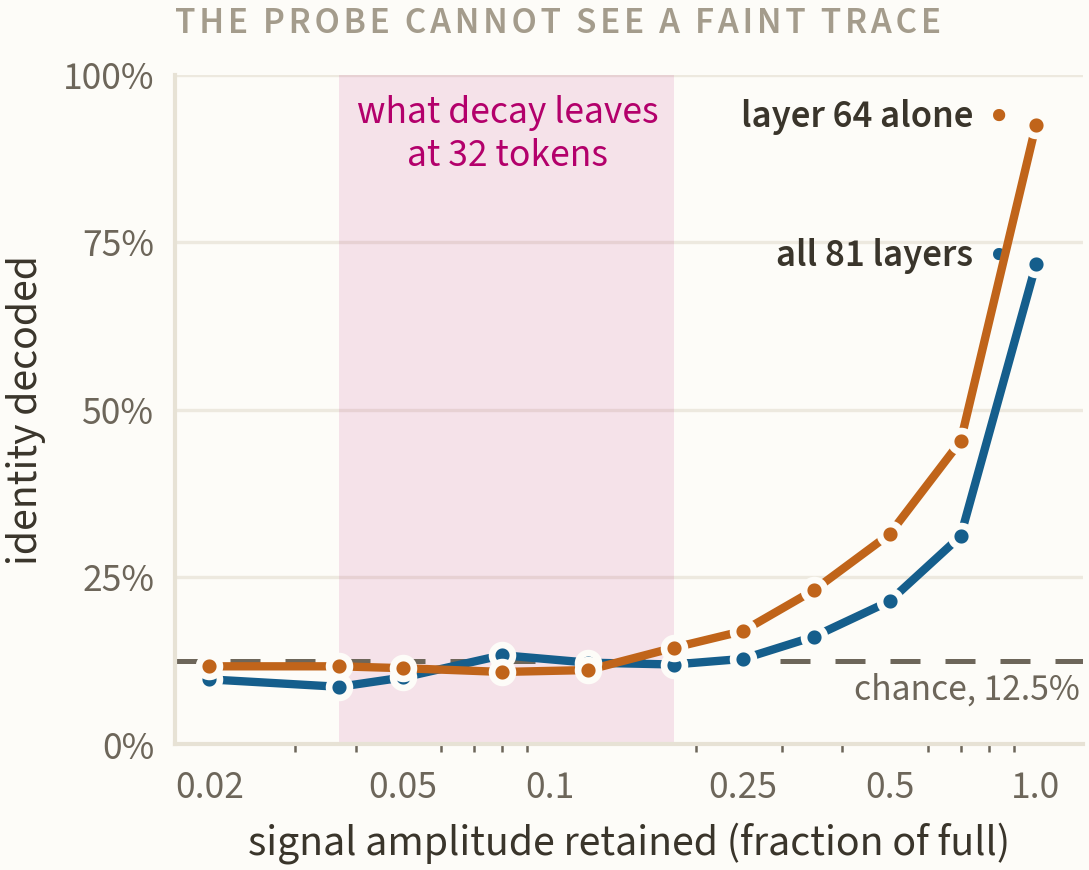
\includegraphics[width=0.72\linewidth]{assets/f4_sensitivity.png}
\caption{How faint a signal the probe can still recover. Each trial's own
contribution is attenuated while an equal amount of unrelated variation is
substituted, holding total variance roughly constant. The shaded band is what
the model's decay parameters leave of a stored trace after 32 tokens, between
the median and the mean over heads. Both probes are at chance throughout that
band, so a visible reading at 32 tokens cannot be a retained one.}
\label{fig:sensitivity}
\end{figure}

\keyfinding{The probe's insensitivity to faint signals is what makes the
positive reading informative. A signal the instrument can see at thirty-two
tokens is necessarily a fresh one, because a retained one would be four to six
times below its detection floor.}

The same measurement bounds what we may conclude. Whether faint retained content
persists below the floor is not answerable with this instrument at any distance
beyond a few tokens, so this paper does not claim the state stops storing the
image. It claims that what a probe reads at distance is not retention, and that
it depends causally on the attention channel.

This one measurement explains three earlier puzzles. First, it explains why
the measured horizon exceeds the predicted one, and why the gap grows in
smaller models: the probe was never measuring retention in the first place.
Second, it explains why the tercile split made the fast heads look like the
best retainers: they write hardest, so whatever the attention channel
re-supplies lands in them at the highest amplitude, and holding the write gain
fixed removes that apparent advantage (Section~\ref{sec:strata}). Third, it
supplies the mechanism behind the causal result, which the next section takes
up.

\section{Result 4: Causally, the Answer Follows the Attention Channel}

The probe results say the attention channel supplies what the recurrent state
appears to hold. The splice tests the same claim on the model's own
behaviour, with no probe involved. Recall the setup: two runs see different
images, one memory channel is exchanged between them, and the host run then
answers its question. We admit a pair only if the host and the donor each
answered their own question correctly beforehand, so the ceiling is $100\%$ by
construction. Of 111 attempted pairs, 11 were rejected on that criterion, and
none were rejected for mismatched cache length. Every recurrent swap was
verified to have actually changed the state, 100 of 100.

\begin{table}[h]
\centering\small
\begin{tabular}{lrrr}
\toprule
condition & layers swapped & follows host & follows donor \\
\midrule
no swap                       & 0  & $100/100$ $[96,100]$ & $0/100$ $[0,4]$ \\
recurrent, all 81 states      & 0  & $100/100$ $[96,100]$ & $0/100$ $[0,4]$ \\
\addlinespace
attention, 1 layer            & 1  & $100/100$ $[96,100]$ & $0/100$ $[0,4]$ \\
attention, 3 layers spread    & 3  & $98/100$ $[93,99]$   & $0/100$ $[0,4]$ \\
attention, 7 layers           & 7  & $4/100$ $[2,10]$     & $94/100$ $[88,97]$ \\
attention, all 13             & 13 & $0/100$ $[0,4]$      & $98/100$ $[93,99]$ \\
\addlinespace
attention, earliest 3         & 3  & $94/100$ $[88,97]$   & $1/100$ $[0,5]$ \\
attention, latest 3           & 3  & $100/100$ $[96,100]$ & $0/100$ $[0,4]$ \\
both channels                 & 13 & $0/100$ $[0,4]$      & $100/100$ $[96,100]$ \\
\bottomrule
\end{tabular}
\caption{The splice at 100 pairs with a $100\%$ ceiling. Brackets are $95\%$
Wilson intervals in percent. Replacing the entire recurrent memory of all 81
layers changes nothing; replacing seven of the thirteen attention caches flips
the answer to the other image.}
\label{tab:splice}
\end{table}

\begin{figure}[h]
\centering
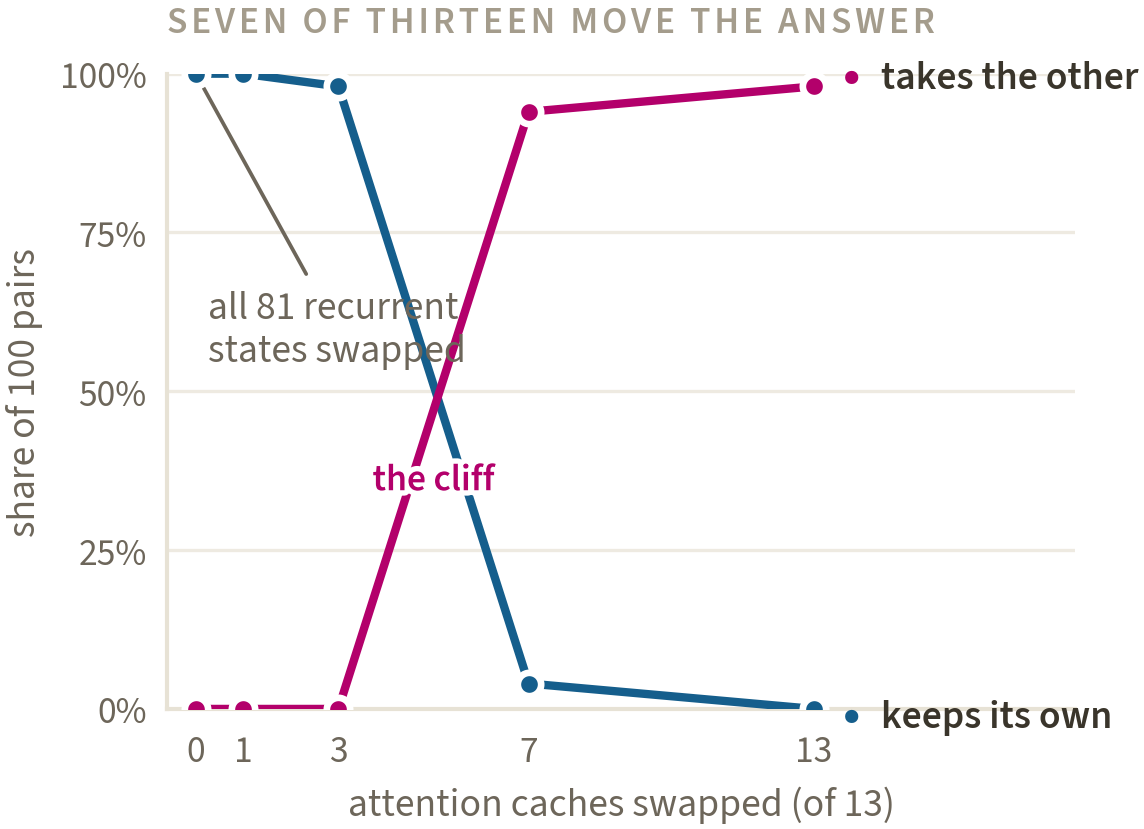
\includegraphics[width=0.72\linewidth]{assets/f5_splice.png}
\caption{How many of the thirteen attention caches must be exchanged before
the answer follows the other image, over 100 pairs in which both images were
answered correctly beforehand. The leftmost point is the recurrent swap: all
81 states replaced, no attention cache touched, no effect. Then notice the
cliff: one swapped cache changes nothing, three change almost nothing, and
seven flip nearly every answer.}
\label{fig:splice}
\end{figure}

Figure~\ref{fig:splice} draws the same result as a curve, and three things
can be read from it. First, replacing the recurrent memory has no effect at
all: exchanging all 81 recurrent states and convolution buffers leaves $100$
of $100$ answers following the host's own image, with every swap verified to
have taken effect. Second, the attention channel is causally sufficient to
determine the answer: swapping seven of the thirteen caches moves $94$ of
$100$ answers to the donor's image. Third, the dependence on attention is
graded and distributed. One swapped attention layer changes nothing, three
spread across the stack move two answers, and seven move almost all of them.
No small subset of layers is enough, so the picture is held across the
attention layers rather than concentrated in a few. The earliest three layers
have a small effect and the latest three have none, which matches the earlier
finding that visual information enters early and is consumed downstream.

Why does replacing 37 million recurrent numbers change nothing? Result 3
already answers this. The transplanted state is decayed away within a few
tokens and rewritten from the attention channel, which the recurrent swap
leaves untouched. The probe result and the splice result are the same fact
seen from two sides.
\section{Result 5: Scale, and Where the Prediction Fails}
\label{sec:scale}

We repeated the core protocol at three model scales. The instruments read
every tensor shape from the loaded model's configuration rather than assuming
the 7B geometry. This is a requirement, not a convenience: the 2.7B and 1.2B
checkpoints use a single B/C group where the 7B uses two, and the 1.2B has a
state dimension of 128 where the others have 64. Table~\ref{tab:scale}
reports the results.

\begin{table}[h]
\centering\small
\begin{tabular}{lrrrrrr}
\toprule
model & layers & attn & probe $d{=}0$ & probe $d{=}64$ & measured $t_{1/2}$ & predicted $t_{1/2}$ \\
\midrule
Zamba2-VL-7B   & 81 & 13 & $71.7\%$ & $21.7\%$ & $4.0$  & $6.64$ \\
Zamba2-VL-2.7B & 54 &  9 & $84.2\%$ & $31.7\%$ & $9.6$  & $2.91$ \\
Zamba2-VL-1.2B & 38 &  6 & $83.3\%$ & $34.2\%$ & $14.3$ & $2.58$ \\
\bottomrule
\end{tabular}
\caption{The same protocol at three scales, 120 identity trials per distance.
The pre-image control reads exactly $12.5\%$ at every scale. Half-lives are in
tokens: measured is the distance at which above-chance decodability halves,
predicted is the median over heads of $\ln 2/(|A|\bar{\Delta})$.}
\label{tab:scale}
\end{table}

Two conclusions follow. The second is a negative result, and we report it
plainly.

First, the parameter-derived horizon is short at every scale. Median predicted
half-lives are $6.64$, $2.91$ and $2.58$ tokens, and the fraction of heads
with a predicted half-life under 32 tokens is $85.0\%$, $97.9\%$ and $95.6\%$.
Whatever the recurrent state genuinely retains of its own past, it retains it
for single-digit token counts in all three models.

Second, the predicted horizon does not predict the measured one. Across the
three models the two quantities move in opposite directions: the prediction
falls with scale while the measurement rises. On the 7B alone the agreement
looked strong, with measured decodability tracking predicted retention at
$r = 0.973$ across eleven distances. That agreement does not replicate at the
other scales. We therefore do not claim that the decay calculation explains
the measured decay curve. Result 3 already showed why it cannot: the probe at
distance is reading relayed content, not retained content, so its curve is not
governed by the decay parameters.

\section{Result 6: Visual Key-Value Eviction Removes the Only Copy, Eventually}

An image adds hundreds of key-value entries to the attention cache, which
makes vision-language models expensive to serve. Pruning methods make them
cheaper by deleting most of those entries, on the premise that the entries
are redundant: on standard benchmarks, many can be deleted and accuracy
barely moves. Our results explain where that redundancy comes from. It comes
from the relay, and the relay only lasts a few tokens, so the premise should
degrade with distance. We test this directly on the model's own behaviour. We
evict a fraction of the visual key-value entries from all 13 attention layers
immediately after the image is read, let the filler and the question stream
past the pruned cache, and measure the model's accuracy. Retention $\rho$ is
the fraction of visual positions kept, sampled uniformly, and the question is
asked $d$ tokens after the image.

\begin{table}[h]
\centering\small
\begin{tabular}{lrrrr}
\toprule
visual KV retained & $d{=}0$ & $d{=}32$ & $d{=}128$ & $d{=}512$ \\
\midrule
$100\%$ & $97.9\%$ & $95.8\%$ & $100.0\%$ & $97.9\%$ \\
$25\%$  & $91.7\%$ & $95.8\%$ & $95.8\%$  & $91.7\%$ \\
$5\%$   & $87.5\%$ & $77.1\%$ & $75.0\%$  & $64.6\%$ \\
$0\%$   & $64.6\%$ & $37.5\%$ & $31.2\%$  & $22.9\%$ \\
\bottomrule
\end{tabular}
\caption{Behavioural accuracy under visual key-value eviction, against distance
between the image and the question. $n = 48$ per cell, chance $12.5\%$, no
failures. The unpruned row is flat, so distance alone costs nothing.}
\label{tab:eviction}
\end{table}

Read as cost relative to the unpruned baseline at the same distance, the
structure is a clean interaction:

\begin{table}[h]
\centering\small
\begin{tabular}{lrrrr}
\toprule
visual KV retained & $d{=}0$ & $d{=}32$ & $d{=}128$ & $d{=}512$ \\
\midrule
$25\%$ & $6.2$  & $0.0$  & $4.2$  & $6.2$ \\
$5\%$  & $10.4$ & $18.8$ & $25.0$ & $33.3$ \\
$0\%$  & $33.3$ & $58.3$ & $68.8$ & $75.0$ \\
\bottomrule
\end{tabular}
\caption{Accuracy points lost to pruning, relative to the unpruned baseline at
the same distance.}
\label{tab:eviction_cost}
\end{table}

Figure~\ref{fig:eviction} plots the four retention levels against distance.
With a quarter of the entries retained, there is no distance effect at all:
the cost is $6.2$, $0.0$, $4.2$ and $6.2$ points, flat within noise. At that
level the redundancy premise holds on this architecture, and we found no
evidence against it.

Below that level, distance starts to matter, and it matters a great deal. At a
twentieth retained, the cost triples across the range, from $10.4$ points
beside the image to $33.3$ points at 512 tokens. With every visual entry
removed, it runs from $33.3$ to $75.0$. Compare the unpruned row, which is
flat across the same distances. So the problem is not that long prompts are
hard. The problem is that long prompts become hard \emph{once the visual
entries are gone}, because by then the recurrent channel has nothing left to
relay from.

\begin{figure}[h]
\centering

\includegraphics[width=0.72\linewidth]{assets/f6_eviction.png}
\caption{Model accuracy under visual key-value eviction, against how far the
question sits from the image, $n = 48$ per point. The unpruned line is flat, so
distance alone costs nothing. Keeping a quarter of the entries is also flat.
Below that the lines fan out: the cost of pruning grows with distance only once
the recurrent channel has stopped relaying the picture.}
\label{fig:eviction}
\end{figure}

\keyfinding{The cost of heavy pruning is not one number. Above a retention
threshold, somewhere between a quarter and a twentieth on this model, pruning
costs the same at every distance. Below it, the cost grows with how far the
question sits from the image: a method validated at short range will
understate its cost at long range by a factor of three at $5\%$ retention.}

The zero-retention row also gives us the cleanest available measure of what
the recurrent channel contributes on its own. With no visual entries anywhere
in the attention caches, the model can only be answering from its recurrent
states. Its accuracy falls from $64.6\%$ beside the image to $22.9\%$ at 512
tokens. That decline is the recurrent channel's own contribution decaying,
measured on behaviour, with an instrument entirely independent of the probe.
It agrees with the picture the probe gives.

One discrepancy should be stated plainly. At zero retention the model still
answers at $37.5\%$ at thirty-two tokens, well above the $12.5\%$ chance rate,
while our linear probe reads the recurrent state at close to chance at that
distance. So the model is using something in the recurrent channel that the
probe does not recover. This means the probe is a lower bound on what the
state carries, not a full measure of it. The sentence ``the state is empty''
is not supported by our evidence, and we do not claim it.

\section{Limitations}
\label{sec:limits}

We separate three kinds of limitation: alternative explanations our evidence
does not exclude, limits on what the instruments can see, and limits on scope.
The first kind is the one that should decide how much weight a reader puts on
the central claim, so it comes first.

\subsection{Alternative explanations we have not excluded}

\textbf{Eviction changes more than the image's presence, though the matched
control argues against this.} Removing the visual key-value entries shortens
every attention layer's cache by roughly 400 positions, and it changes the
softmax normalisation for every token that follows. Section~\ref{sec:controls}
reports the matched control: deleting an equal number of \emph{non-visual}
positions from the same caches. The two deletions move the readout in opposite
directions, which pure damage cannot produce. A narrower version of the worry
survives. The pre-image text we remove does not contribute to the residual
stream in the same way the image does, so the comparison bounds the damage
account rather than eliminating every version of it.

\textbf{The relay result could be a sensitivity asymmetry. We bound this but
do not eliminate it.} Our own data show the probe is a lower bound (see
below), and a lower bound need not be uniform. Freshly re-encoded content
plausibly sits at higher amplitude than content written many tokens earlier
and decayed. If the probe recovers strong signals easily and weak signals
poorly, removing the re-encoded copy could collapse the readout even in a
state that still retained something. Section~\ref{sec:sensitivity} answers
this by measuring the probe's detection floor and showing that predicted
retention at thirty-two tokens sits below that floor, so a visible reading
there cannot be a retained one. This argument makes one assumption: that
decay followed by overwriting weakens the discriminative signal roughly the
way our attenuation procedure does. A model with no attention channel to
relay from would settle the question without that assumption, and we have not
tested one.

\textbf{The route is located but not traced.} The layerwise eviction of
Section~\ref{sec:controls} shows the relay enters early: zeroing the three
earliest attention layers reproduces $15.8$ of the $17.2$ points lost when all
thirteen are zeroed, while the three latest produce $0.5$. What is not traced is
the intermediate path, from attention output through the residual stream into a
downstream mixer's write.

\subsection{What the instruments can and cannot see}

\textbf{The probe is a lower bound, and our own behavioural data prove it.}
With every visual key-value entry removed, the model answers at $37.5\%$ at
thirty-two tokens while the probe reads the recurrent state near chance at the
same distance. Something usable survives there that a 512-dimensional random
projection, read by a linear probe trained on 120 examples, does not recover.
Every statement in this paper about what the state contains should be read as a
statement about what is linearly decodable under that instrument. This paper does
not establish that the state is empty of the image at any distance, and makes no
such claim.

\textbf{Probe accuracy depends on the feature-to-trial ratio.} Count read at
chance with 128 projection features and reached $19.4\%$ at 512. In the other
direction, the full $41{,}472$-dimensional state probe reads $71.7\%$ where a
single layer's 512 features read $92.5\%$ on identical trials. Absolute
accuracies are therefore not comparable across collections of different size or
width, and we report them only within a collection. The decay curve in
Table~\ref{tab:fine} is internally consistent because the same 120 trials appear
at every distance.

\textbf{One projection basis for most results.} The eviction contrast was
repeated across three independent Gaussian projection bases and is stable under
them (fast tercile at $d{=}32$: intact $31.2 \pm 1.6\%$ against evicted
$9.9 \pm 1.8\%$, mean and standard deviation over seeds). The decay-curve
collections still use a single fixed basis, so the variance attributable to the
choice of basis is unmeasured there.

\textbf{The stratum dose-response is confirmed at matched amplitude only at
distance zero, in one model.} On splits by half-life the eviction sensitivity
is ordered exactly by predicted decay rate: $37.5$, $18.8$ and $7.8$ points
over terciles ($r = 0.991$), and $r = 0.800$ ($95\%$ CI $[0.34, 0.95]$) at
$32$ tokens over deciles with about $6$ points of binomial noise per cell at
$n = 64$. But every split by half-life is also a split by write amplitude, and
the amplitude-controlled version is thinner: a $2.4\times$ ratio at distance
zero over two strata at $n = 192$, and no measurement at thirty-two tokens,
where the gain-matched fast stratum reads too close to chance intact for
eviction to have anything to remove. Two strata at one distance in one model
is a direction, not a curve.

\subsection{Scope}

\textbf{One model family, and a second family we tried and failed on.} Results
come from three Zamba2-VL checkpoints, which is one vendor, one architecture
family and one training recipe. This is the principal limit on the paper's
generality.

We attempted to extend the relay result to a second family and report the
attempt because its failure is informative. Granite 4.0 h-tiny \cite{granite4} is a Mamba2
hybrid from a different lineage, with 36 recurrent layers to 4 attention layers
against Zamba2-VL-7B's 81 to 13. Its decay parameters read out cleanly and give
a median predicted half-life of $8.7$ tokens, so the horizon calculation of
Section 5 transfers to a second family. The relay contrast does not, for an
instrumental reason: on a code-word recall task the model answers correctly on
$100\%$, $96.9\%$ and $100\%$ of trials at $0$, $32$ and $64$ tokens, and yet a
probe on its recurrent state reads at chance at distance zero. Scaling to 256
trials did not change this ($13.7\%$ against a $12.5\%$ chance rate,
$p = 0.31$), and neither did probing single layers, where the best of 36 layers
reached $19.9\%$.

We suspected the item was too small to write a detectable trace, a one-token
code word against a 345-token image, and tested that by repeating the carrier
sixteen times so the item occupied 192 tokens. It did not help: $12.0\%$,
$17.2\%$ and $10.9\%$ across the three strata. Repetition lengthens an item
without diversifying what it writes, so the state ends up holding little more
than the final repeat, which is not the manipulation we intended. We do not
know why the instrument fails on this model; we only know that it does. No
relay claim can be made beyond the Zamba2-VL family on this evidence. A vision-language hybrid from a second family, where the item
is a real image, remains the right test and we have not run it. The sharper
version of that test is a vision-language model with no attention layers at all,
such as Cobra \cite{zhao2025cobra} or VL-Mamba \cite{qiao2024vlmamba}, where
probing the recurrent state must be measuring retention because there is nothing
else it could be measuring. Both are Mamba1 models and would need the read
operator ported before any number from them could be trusted.

\textbf{One task format, one dataset, one modality.} Eight-way forced choice on
COCO buys an exact chance rate and a clean pre-image control, and costs
generality to free-form answering, to other visual properties, and to whether
any of this holds for text held in the same states.

\textbf{The horizon is measured on one filler distribution.} $\bar{\Delta}$ is
input dependent. We measured it on natural prose and found the median half-life
stable across images, from $6.44$ to $6.86$ tokens, but a filler with very
different gate statistics would give a different horizon, which the same
calculation would predict.
\section{Conclusion}

The recurrent state of this hybrid vision-language model is not a memory of
the image in any useful sense. It is a selective summary of the picture's
gist, and it holds that summary for only a few tokens. This lifetime is not an
empirical curiosity: it can be computed from the model's own decay parameters
before any measurement is taken. What the model actually answers from lives in
the thin attention channel, and the recurrent state relays that content
rather than storing its own copy. The practical consequence is direct: the
visual key-value entries a hybrid carries are redundant only for as long as
the recurrent state is still relaying the picture, and that is not long.

\begin{thebibliography}{99}\small\setlength{\itemsep}{1pt}

\bibitem{katharopoulos2020linear}
A.~Katharopoulos, A.~Vyas, N.~Pappas, and F.~Fleuret.
\newblock Transformers are RNNs: Fast Autoregressive Transformers with Linear
Attention. \emph{ICML}, 2020.

\bibitem{gu2022s4}
A.~Gu, K.~Goel, and C.~R\'e.
\newblock Efficiently Modeling Long Sequences with Structured State Spaces.
\emph{ICLR}, 2022.

\bibitem{peng2023rwkv}
B.~Peng, E.~Alcaide, Q.~Anthony, A.~Albalak, S.~Arcadinho, S.~Biderman, et~al.
\newblock RWKV: Reinventing RNNs for the Transformer Era.
\emph{arXiv:2305.13048}, 2023.

\bibitem{gu2023mamba}
A.~Gu and T.~Dao.
\newblock Mamba: Linear-Time Sequence Modeling with Selective State Spaces.
\emph{arXiv:2312.00752}, 2023.

\bibitem{dao2024mamba2}
T.~Dao and A.~Gu.
\newblock Transformers are SSMs: Generalized Models and Efficient Algorithms
Through Structured State Space Duality. \emph{ICML}, 2024.

\bibitem{beck2024xlstm}
M.~Beck, K.~P\"oppel, M.~Spanring, A.~Auer, O.~Prudnikova, M.~Kopp,
G.~Klambauer, J.~Brandstetter, and S.~Hochreiter.
\newblock xLSTM: Extended Long Short-Term Memory.
\emph{arXiv:2405.04517}, 2024.

\bibitem{lieber2024jamba}
O.~Lieber, B.~Lenz, H.~Bata, G.~Cohen, J.~Osin, I.~Dalmedigos, et~al.
\newblock Jamba: A Hybrid Transformer-Mamba Language Model.
\emph{arXiv:2403.19887}, 2024.

\bibitem{glorioso2024zamba}
P.~Glorioso, Q.~Anthony, Y.~Tokpanov, J.~Whittington, J.~Pilault, A.~Ibrahim,
and B.~Millidge.
\newblock Zamba: A Compact 7B SSM Hybrid Model.
\emph{arXiv:2405.16712}, 2024.

\bibitem{de2024griffin}
S.~De, S.~L. Smith, A.~Fernando, A.~Botev, G.~Cristian-Muraru, A.~Gu, et~al.
\newblock Griffin: Mixing Gated Linear Recurrences with Local Attention for
Efficient Language Models. \emph{arXiv:2402.19427}, 2024.

\bibitem{ren2025samba}
L.~Ren, Y.~Liu, Y.~Lu, Y.~Shen, C.~Liang, and W.~Chen.
\newblock Samba: Simple Hybrid State Space Models for Efficient Unlimited
Context Language Modeling. \emph{ICLR}, 2025.

\bibitem{waleffe2024empirical}
R.~Waleffe, W.~Byeon, D.~Riach, B.~Norick, V.~Korthikanti, T.~Dao, A.~Gu,
et~al.
\newblock An Empirical Study of Mamba-based Language Models.
\emph{arXiv:2406.07887}, 2024.

\bibitem{jelassi2024copying}
S.~Jelassi, D.~Brandfonbrener, S.~M. Kakade, and E.~Malach.
\newblock Repeat After Me: Transformers are Better than State Space Models at
Copying. \emph{arXiv:2402.01032}, 2024.

\bibitem{merrill2024illusion}
W.~Merrill, J.~Petty, and A.~Sabharwal.
\newblock The Illusion of State in State-Space Models. \emph{ICML}, 2024.

\bibitem{wen2024rnns}
K.~Wen, X.~Dang, and K.~Lyu.
\newblock RNNs are not Transformers (Yet): The Key Bottleneck on In-context
Retrieval. \emph{arXiv:2402.18510}, 2024.

\bibitem{arora2023zoology}
S.~Arora, S.~Eyuboglu, A.~Timalsina, I.~Johnson, M.~Poli, J.~Zou, A.~Rudra,
and C.~R\'e.
\newblock Zoology: Measuring and Improving Recall in Efficient Language Models.
\emph{arXiv:2312.04927}, 2023.

\bibitem{arora2024based}
S.~Arora, S.~Eyuboglu, M.~Zhang, A.~Timalsina, S.~Alberti, D.~Zinsley, J.~Zou,
A.~Rudra, and C.~R\'e.
\newblock Simple Linear Attention Language Models Balance the Recall-Throughput
Tradeoff. \emph{arXiv:2402.18668}, 2024.

\bibitem{alain2016probes}
G.~Alain and Y.~Bengio.
\newblock Understanding Intermediate Layers Using Linear Classifier Probes.
\emph{arXiv:1610.01644}, 2016.

\bibitem{hewitt2019control}
J.~Hewitt and P.~Liang.
\newblock Designing and Interpreting Probes with Control Tasks.
\emph{EMNLP}, 2019.

\bibitem{belinkov2022probing}
Y.~Belinkov.
\newblock Probing Classifiers: Promises, Shortcomings, and Advances.
\emph{Computational Linguistics}, 2022.

\bibitem{vig2020causal}
J.~Vig, S.~Gehrmann, Y.~Belinkov, S.~Qian, D.~Nevo, S.~Sakenis, J.~Huang,
Y.~Singer, and S.~Shieber.
\newblock Causal Mediation Analysis for Interpreting Neural NLP: The Case of
Gender Bias. \emph{arXiv:2004.12265}, 2020.

\bibitem{meng2022rome}
K.~Meng, D.~Bau, A.~Andonian, and Y.~Belinkov.
\newblock Locating and Editing Factual Associations in GPT.
\emph{NeurIPS}, 2022.

\bibitem{wang2022ioi}
K.~Wang, A.~Variengien, A.~Conmy, B.~Shlegeris, and J.~Steinhardt.
\newblock Interpretability in the Wild: a Circuit for Indirect Object
Identification in GPT-2 small. \emph{arXiv:2211.00593}, 2022.

\bibitem{zhang2024patching}
F.~Zhang and N.~Nanda.
\newblock Towards Best Practices of Activation Patching in Language Models:
Metrics and Methods. \emph{ICLR}, 2024.

\bibitem{chen2024fastv}
L.~Chen, H.~Zhao, T.~Liu, S.~Bai, J.~Lin, C.~Zhou, and B.~Chang.
\newblock An Image is Worth 1/2 Tokens After Layer 2: Plug-and-Play Inference
Acceleration for Large Vision-Language Models. \emph{ECCV}, 2024.

\bibitem{yang2024visionzip}
S.~Yang, Y.~Chen, Z.~Tian, C.~Wang, J.~Li, B.~Yu, and J.~Jia.
\newblock VisionZip: Longer is Better but Not Necessary in Vision Language
Models. \emph{arXiv:2412.04467}, 2024.

\bibitem{shang2025prumerge}
Y.~Shang, M.~Cai, B.~Xu, Y.~J. Lee, and Y.~Yan.
\newblock LLaVA-PruMerge: Adaptive Token Reduction for Efficient Large
Multimodal Models. \emph{ICCV}, 2025.

\bibitem{zhang2023h2o}
Z.~Zhang, Y.~Sheng, T.~Zhou, T.~Chen, L.~Zheng, R.~Cai, Z.~Song, Y.~Tian,
C.~R\'e, C.~Barrett, Z.~Wang, and B.~Chen.
\newblock H\textsubscript{2}O: Heavy-Hitter Oracle for Efficient Generative
Inference of Large Language Models. \emph{arXiv:2306.14048}, 2023.

\bibitem{li2024snapkv}
Y.~Li, Y.~Huang, B.~Yang, B.~Venkitesh, A.~Locatelli, H.~Ye, T.~Cai, P.~Lewis,
and D.~Chen.
\newblock SnapKV: LLM Knows What You are Looking for Before Generation.
\emph{arXiv:2404.14469}, 2024.

\bibitem{xiao2024streaming}
G.~Xiao, Y.~Tian, B.~Chen, S.~Han, and M.~Lewis.
\newblock Efficient Streaming Language Models with Attention Sinks.
\emph{ICLR}, 2024.

\bibitem{liu2023llava}
H.~Liu, C.~Li, Q.~Wu, and Y.~J. Lee.
\newblock Visual Instruction Tuning. \emph{NeurIPS}, 2023.

\bibitem{bai2025qwen25vl}
S.~Bai, K.~Chen, X.~Liu, J.~Wang, W.~Ge, S.~Song, et~al.
\newblock Qwen2.5-VL Technical Report. \emph{arXiv:2502.13923}, 2025.

\bibitem{zhao2025cobra}
H.~Zhao, M.~Zhang, W.~Zhao, P.~Ding, S.~Huang, and D.~Wang.
\newblock Cobra: Extending Mamba to Multi-Modal Large Language Model for
Efficient Inference. \emph{AAAI}, 2025.

\bibitem{qiao2024vlmamba}
Y.~Qiao, Z.~Yu, L.~Guo, S.~Chen, Z.~Zhao, M.~Sun, Q.~Wu, and J.~Liu.
\newblock VL-Mamba: Exploring State Space Models for Multimodal Learning.
\emph{arXiv:2403.13600}, 2024.

\bibitem{lin2014coco}
T.-Y. Lin, M.~Maire, S.~Belongie, L.~Bourdev, R.~Girshick, J.~Hays, P.~Perona,
D.~Ramanan, C.~L. Zitnick, and P.~Doll\'ar.
\newblock Microsoft COCO: Common Objects in Context.
\newblock \emph{ECCV}, 2014. arXiv:1405.0312.

\bibitem{zamba2vl}
Zyphra.
\newblock Zamba2-VL-7B model card.
\newblock \url{https://huggingface.co/Zyphra/Zamba2-VL-7B}, 2026. Apache-2.0.

\bibitem{granite4}
IBM Granite Team.
\newblock Granite 4.0 h-tiny model card.
\newblock \url{https://huggingface.co/ibm-granite/granite-4.0-h-tiny}, 2025.

\end{thebibliography}

\end{document}
